\documentclass[tikz,margin=1mm]{standalone}
\usepackage{xcolor}
 \usetikzlibrary{arrows.meta,chains, decorations.pathreplacing}



\begin{document}
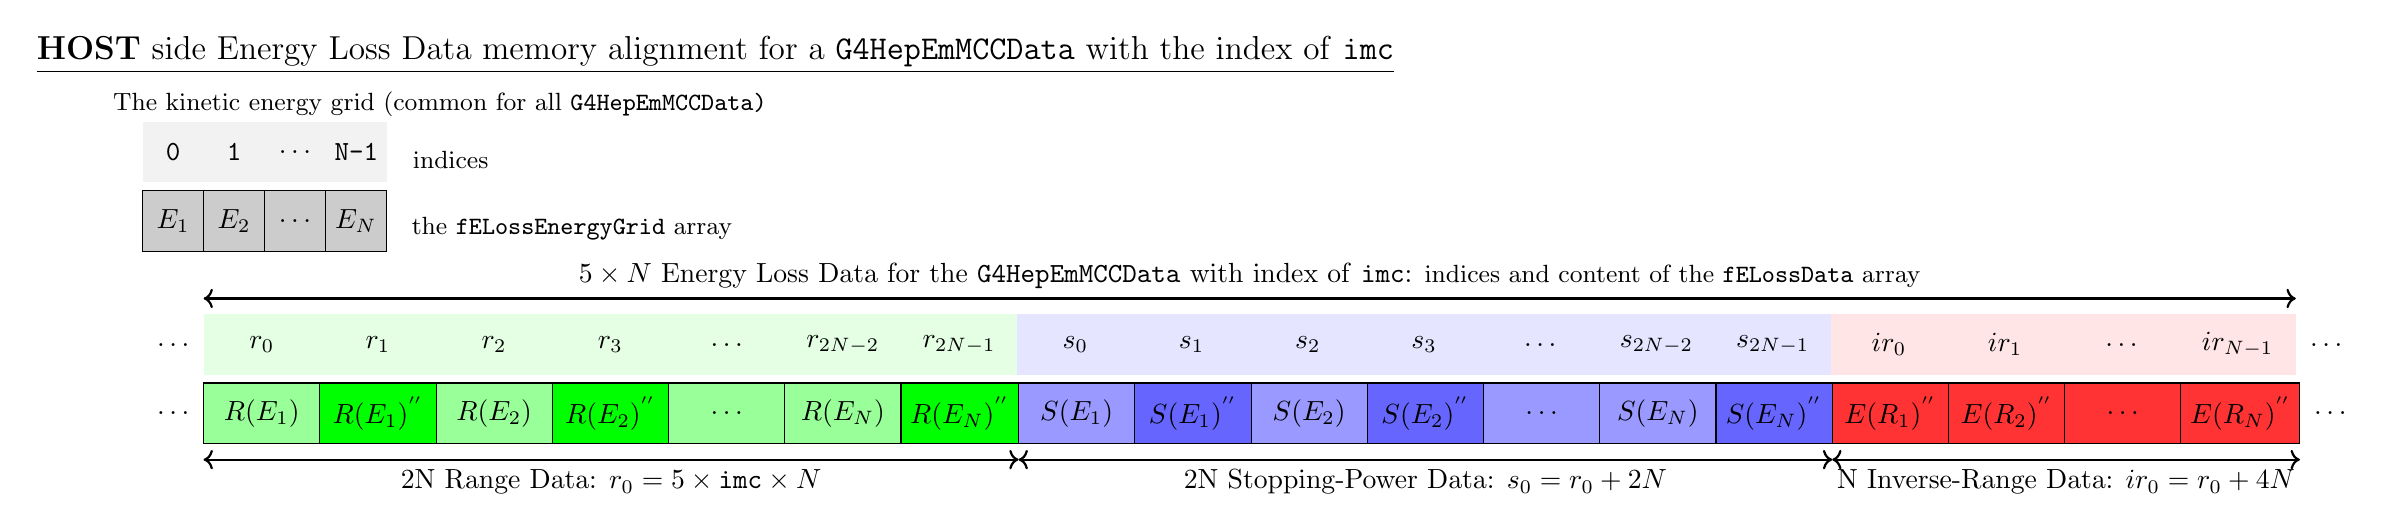
\begin{tikzpicture}[
   start chain       = going right,
   node distance = 0pt,
    %
   noStyle/.style  = {draw=none, minimum width=2.2em, minimum height=2.2em, outer sep=0pt, font=\ttfamily, on chain},
   %
   eiStyle/.style  = {draw=none, minimum width=2.2em, minimum height=2.2em, outer sep=0pt, font=\ttfamily, on chain, fill=gray!10},
   eStyle/.style   = {draw, minimum width=2.2em, minimum height=2.2em, outer sep=0pt, on chain, fill=gray!40},
   %
   riStyle/.style  = {draw=none, minimum width=4.2em, minimum height=2.2em, outer sep=0pt, font=\ttfamily, on chain, fill=green!10},
   rStyle/.style   = {draw, minimum width=4.2em, minimum height=2.2em, outer sep=0pt, on chain, fill=green!40},
   rSDStyle/.style   = {draw, minimum width=4.2em, minimum height=2.2em, outer sep=0pt, on chain, fill=green!100},
   %
   siStyle/.style  = {draw=none, minimum width=4.2em, minimum height=2.2em, outer sep=0pt, font=\ttfamily, on chain, fill=blue!10},
   sSDStyle/.style  = {draw, minimum width=4.2em, minimum height=2.2em, outer sep=0pt, font=\ttfamily, on chain, fill=blue!60},
   sStyle/.style   = {draw, minimum width=4.2em, minimum height=2.2em, outer sep=0pt, on chain, fill=blue!40},
   %
   iriStyle/.style  = {draw=none, minimum width=4.2em, minimum height=2.2em, outer sep=0pt, font=\ttfamily, on chain, fill=red!10},
   irStyle/.style  = {draw, minimum width=4.2em, minimum height=2.2em, outer sep=0pt, font=\ttfamily, on chain, fill=red!80},
  ]

    \begin{scope}[start chain=EGRIDINDX going right];
        \node [eiStyle] (Ei1) {0};
        \node [eiStyle] (Ei2) {1};
        \node [eiStyle] (Ei3) {$\ldots$};
        \node [eiStyle] (Ei4) {N-1};
    \end{scope}

    \node[anchor=north, at={([yshift=+12mm,xshift=+65mm]EGRIDINDX-1.north east)}] {\large {\underline{\textbf{HOST} side Energy Loss Data memory alignment  for a \texttt{G4HepEmMCCData}  with the index of \texttt{imc}} }};
    
    \node[anchor=north, at={([yshift=+5mm,xshift=+30mm]EGRIDINDX-1.north east)}] {\small {The kinetic energy grid (common for all \texttt{G4HepEmMCCData)}}};

    \begin{scope}[start chain=EGRID going right];
        \node [eStyle, anchor=north, at={([yshift=-1mm]EGRIDINDX-1.south)}] (E1) {$E_1$};
        \node [eStyle] (E2) {$E_2$};
        \node [eStyle] (E3) {$\ldots$};
        \node [eStyle] (E4) {$E_N$};
    \end{scope}
    \node[anchor=west, at={([yshift=-1mm,xshift=2mm]EGRIDINDX-4.east)}] {\small {indices}};
    \node[anchor=west, at={([yshift=-1mm,xshift=2mm]EGRID-4.east)}] {\small {the \texttt{fELossEnergyGrid} array}};




    \begin{scope}[start chain=RANGEINDX going right];
        \node [noStyle, anchor=north, at={([yshift=-8mm]EGRID-1.south)}] (Ri1) {$\ldots$};
        \node [riStyle] (Ri2) {$r_0$};
        \node [riStyle] (Ri3) {$r_1$};
        \node [riStyle] (Ri4) {$r_2$};
        \node [riStyle] (Ri5) {$r_3$};
        \node [riStyle] (Ri6) {$\ldots$};
        \node [riStyle] (Ri7) {$r_{2N-2}$};
        \node [riStyle] (Ri8) {$r_{2N-1}$};
    \end{scope}
    
%    \node[anchor=north, at={([yshift=+4mm,xshift=+4.5mm]EGRIDINDX-1.north east)}] {\scriptsize {Kinetic energy grid:}};
%
    \begin{scope}[start chain=RANGE going right];
        \node [noStyle, anchor=north, at={([yshift=-1mm]RANGEINDX-1.south)}] (R1) {$\ldots$};
        \node [rStyle]      (R2) {$R(E_1)$};
        \node [rSDStyle] (R3) {$R(E_1)^{''}$};
        \node [rStyle]     (R4) {$R(E_2)$};
        \node [rSDStyle] (R5) {$R(E_2)^{''}$};
        \node [rStyle]     (E6) {$\ldots$};
        \node [rStyle]    (R7) {$R(E_N)$};
        \node [rSDStyle] (R8) {$R(E_N)^{''}$};
    \end{scope}

   \draw[<->, thick] ([yshift=-2mm]RANGE-2.south west) -- node[below] {2N Range Data: $r_0 = 5\times\texttt{imc}\times N$} ([yshift=-2mm]RANGE-8.south east);





    \begin{scope}[start chain=SPINDX going right];
        \node [siStyle, anchor=west, at={(RANGEINDX-8.east)}] (Si1) {$s_0$};
        \node [siStyle] (Si2) {$s_1$};
        \node [siStyle] (Si3) {$s_2$};
        \node [siStyle] (Si4) {$s_3$};
        \node [siStyle] (Si5) {$\ldots$};
        \node [siStyle] (Si6) {$s_{2N-2}$};
        \node [siStyle] (Si7) {$s_{2N-1}$};
    \end{scope}
    
%    \node[anchor=north, at={([yshift=+4mm,xshift=+4.5mm]EGRIDINDX-1.north east)}] {\scriptsize {Kinetic energy grid:}};
%
    \begin{scope}[start chain=SP going right];
        \node [sStyle, anchor=west, at={(RANGE-8.east)}] (S1) {$S(E_1)$};
        \node [sSDStyle] (S2) {$S(E_1)^{''}$};
        \node [sStyle] (S3) {$S(E_2)$};
        \node [sSDStyle] (S4) {$S(E_2)^{''}$};
        \node [sStyle] (S5) {$\ldots$};
        \node [sStyle] (S6) {$S(E_N)$};
        \node [sSDStyle] (S7) {$S(E_N)^{''}$};
    \end{scope}

   \draw[<->, thick] ([yshift=-2mm]SP-1.south west) -- node[below] {2N Stopping-Power Data: $s_0=r_0+2N$} ([yshift=-2mm]SP-7.south east);



    \begin{scope}[start chain=IRINDX going right];
        \node [iriStyle, anchor=west, at={(SPINDX-7.east)}] (IRi1) {$ir_0$};
        \node [iriStyle] (IRi2) {$ir_1$};
        \node [iriStyle] (IRi3) {$\ldots$};
        \node [iriStyle] (IRi4) {$ir_{N-1}$};
        \node [noStyle] (IRi5) {$\ldots$};
    \end{scope}
    
    \begin{scope}[start chain=IR going right];
        \node [irStyle, anchor=west, at={(SP-7.east)}] (IR1) {$E(R_1)^{''}$};
        \node [irStyle] (IR2) {$E(R_2)^{''}$};
        \node [irStyle] (IR3) {$\ldots$};
        \node [irStyle] (IR4) {$E(R_N)^{''}$};
        \node [noStyle] (IR5) {$\ldots$};
    \end{scope}

   \draw[<->, thick] ([yshift=-2mm]IR-1.south west) -- node[below] {N Inverse-Range Data: $ir_0 = r_0 + 4N$} ([yshift=-2mm]IR-4.south east);


   \draw[<->, thick] ([yshift=+2mm]RANGEINDX-2.north west) -- node[above] {$5\times N$ Energy Loss Data for the \texttt{G4HepEmMCCData} with index of \texttt{imc}: \small {indices and content of the \texttt{fELossData} array}} ([yshift=+2mm]IRINDX-4.north east);


%    \node[anchor=west, at={([yshift=-1mm,xshift=2mm]IRINDX-5.east)}] {\small {indices}};
 %   \node[anchor=west, at={([yshift=-1mm,xshift=2mm]IR-5.east)}] {\small {the \texttt{fELossData} array}};



\end{tikzpicture}
\end{document}
